\section*{Introduction}
\begin{frame}{Contexte}
  \begin{small}
    \begin{quote}
      Toute information utilisée pour caractériser une entité. 
      %Une entité est une personne, un lieu, ou un objet. 
    \end{quote}
  \end{small}
\vfill

  \begin{minipage}{.48\linewidth}
\begin{coloredbox}[black]{Dimensions de contexte}
    %Dimensions de contexte:
    %\begin{itemize}
     Monde physique (état matériel). %localisation géographique
\vfill
     Monde logiciel (agenda).
\vfill
     L'utilisateur (mesures \\physiologiques).
\vfill
     Activités de l'utilisateur (ouverture de porte).
    %\end{itemize}
\end{coloredbox}
  \end{minipage}
  \hfill
  \begin{minipage}{.48\linewidth}
\begin{coloredbox}[black]{ Services \textbf{sensibles au contexte}}
    %Services \textbf{sensibles au contexte}: 
    Utiliser le contexte. 
    \vfill 
    Interagir avec l'utilisateur.
\end{coloredbox}
  \end{minipage}
\end{frame}


\begin{frame}{Sensibilité au contexte pour supporter l'autonomie domiciliaire}
  Services sensibles au contexte définis par des {\bf experts du domaine}:
  \vfill
  \begin{minipage}{.3\linewidth}
\onslide<2->{
    \begin{coloredbox}[black]{Préparer le déjeuner}
      Allumer le four.
      \\
      Ouvrir le frigidaire.
    \end{coloredbox}
}
  \end{minipage}
  \hfill
  \begin{minipage}{.3\linewidth}
\onslide<3->{
    \begin{coloredbox}[black]{Lever}
      Présence dans la chambre.
      \\
      Présence dans la cuisine.
    \end{coloredbox}
}
  \end{minipage}
  \hfill
  \begin{minipage}{.3\linewidth}
\onslide<4->{
    \begin{coloredbox}[black]{Porte entrée ouverte non surveillée}
      Ouvrir la porte d'entrée.
      \\
      Absence dans \\l'entrée.
    \end{coloredbox}
}
  \end{minipage}
  \vfill
% \onslide<5->{
%   Domaine applicatif idéal, mais il y a un certain nombre de défis.
% }
\end{frame}

\begin{frame}{Défis de l'autonomie domiciliaire}
\vspace*{-6.3mm}
\begin{minipage}{.4\linewidth}
\small
Fiabilité de la détection du contexte. 
\\
Multiples axes de variation 
\begin{scriptsize}
(Utilisateurs, domiciles, intervenants).
\end{scriptsize}

Dynamicité.
\end{minipage}
\hfill
\begin{minipage}{.5\linewidth}
    
\includegraphics[scale=0.1]{axe_variation_nill.png}
\end{minipage}
\vfill
% \onslide<2->{
%   \begin{coloredbox}[red]{Problématique}
% \centering
%    Comment couvrir les besoins des services sensibles au contexte?
%   \end{coloredbox}
% }
\end{frame}

\begin{frame}{Défis de l'autonomie domiciliaire}
  \addtocounter{framenumber}{-1}
\vspace*{-6.3mm}
\begin{minipage}{.4\linewidth}
\small
Fiabilité de la détection du contexte. 
\\
Multiples axes de variation 
\begin{scriptsize}
(Utilisateurs, domiciles, intervenants).
\end{scriptsize}

Dynamicité.
\end{minipage}
\hfill
\begin{minipage}{.5\linewidth}
    
\includegraphics[scale=0.1]{axe_variation_1.png}
\end{minipage}
\vfill
% \onslide<2->{
%   \begin{coloredbox}[red]{Problématique}
% \centering
%    Comment couvrir les besoins des services sensibles au contexte?
%   \end{coloredbox}
% }
\end{frame}

\begin{frame}{Défis de l'autonomie domiciliaire}
  \addtocounter{framenumber}{-1}
\vspace*{-6.3mm}
\begin{minipage}{.4\linewidth}
\small
Fiabilité de la détection du contexte. 
\\
Multiples axes de variation 
\begin{scriptsize}
(Utilisateurs, domiciles, intervenants).
\end{scriptsize}

Dynamicité.
\end{minipage}
\hfill
\begin{minipage}{.5\linewidth}
    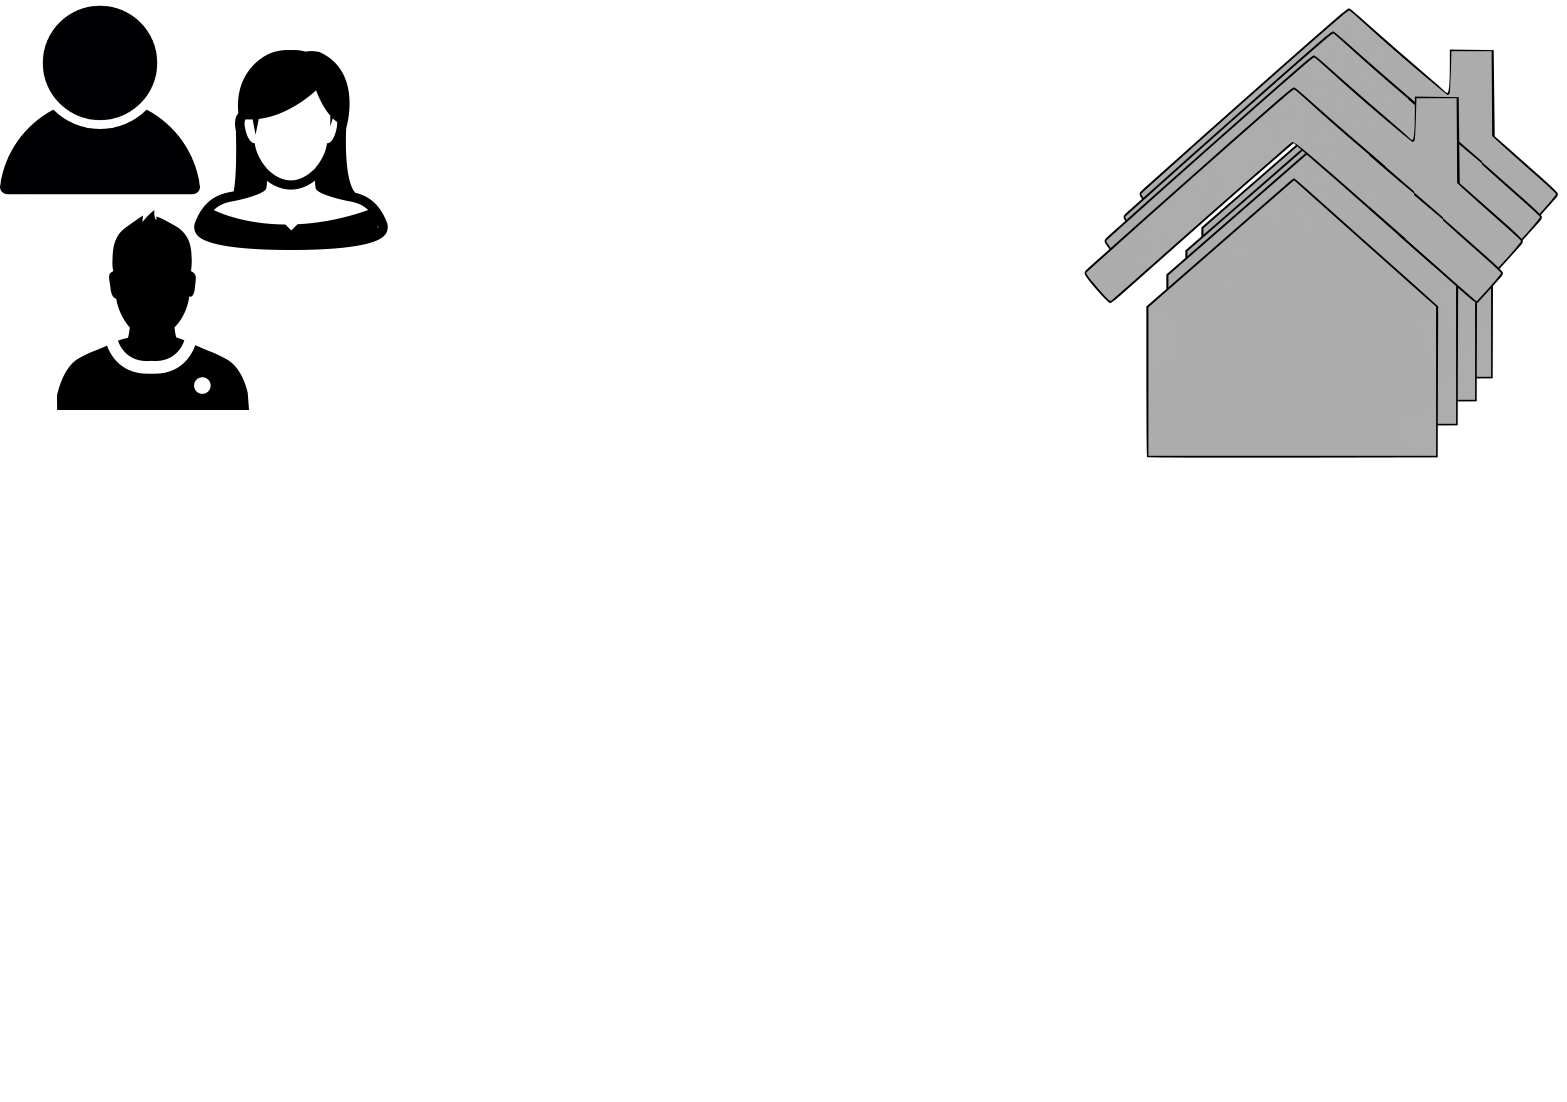
\includegraphics[scale=0.1]{axe_variation_2.png}
\end{minipage}
\vfill
% \onslide<2->{
%   \begin{coloredbox}[red]{Problématique}
% \centering
%    Comment couvrir les besoins des services sensibles au contexte?
%   \end{coloredbox}
% }
\end{frame}

\begin{frame}{Défis de l'autonomie domiciliaire}
  \addtocounter{framenumber}{-1}
\vspace*{-6.3mm}
\begin{minipage}{.4\linewidth}
\small
Fiabilité de la détection du contexte. 
\\
Multiples axes de variation 
\begin{scriptsize}
(Utilisateurs, domiciles, intervenants).
\end{scriptsize}

Dynamicité.
\end{minipage}
\hfill
\begin{minipage}{.5\linewidth}
    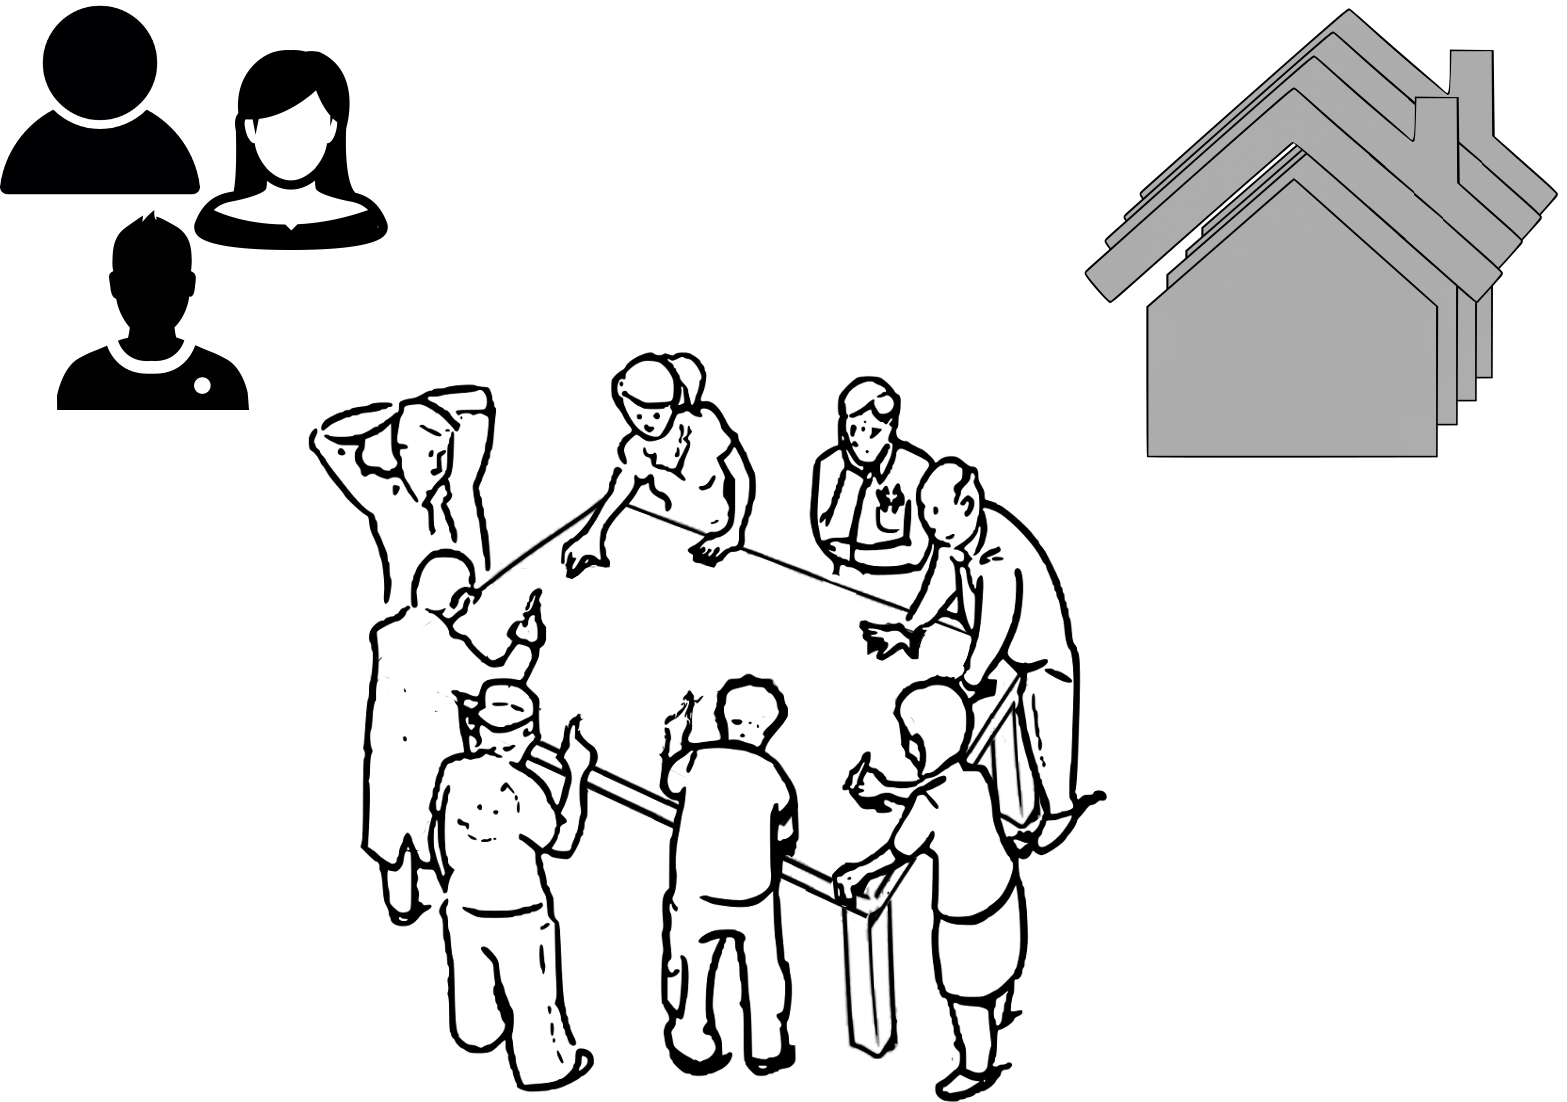
\includegraphics[scale=0.1]{axe_variation_int.png}
\end{minipage}
\vfill
% \onslide<2->{
%   \begin{coloredbox}[red]{Problématique}
% \centering
%    Comment couvrir les besoins des services sensibles au contexte?
%   \end{coloredbox}
% }
\end{frame}

\begin{frame}{Défis de l'autonomie domiciliaire}
  \addtocounter{framenumber}{-1}
\begin{minipage}{.4\linewidth}
\small
Fiabilité de la détection du contexte. 
\\
Multiples axes de variation 
\begin{scriptsize}
(Utilisateurs, domiciles, intervenants).
\end{scriptsize}

Dynamicité.
\end{minipage}
\hfill
\begin{minipage}{.5\linewidth}
    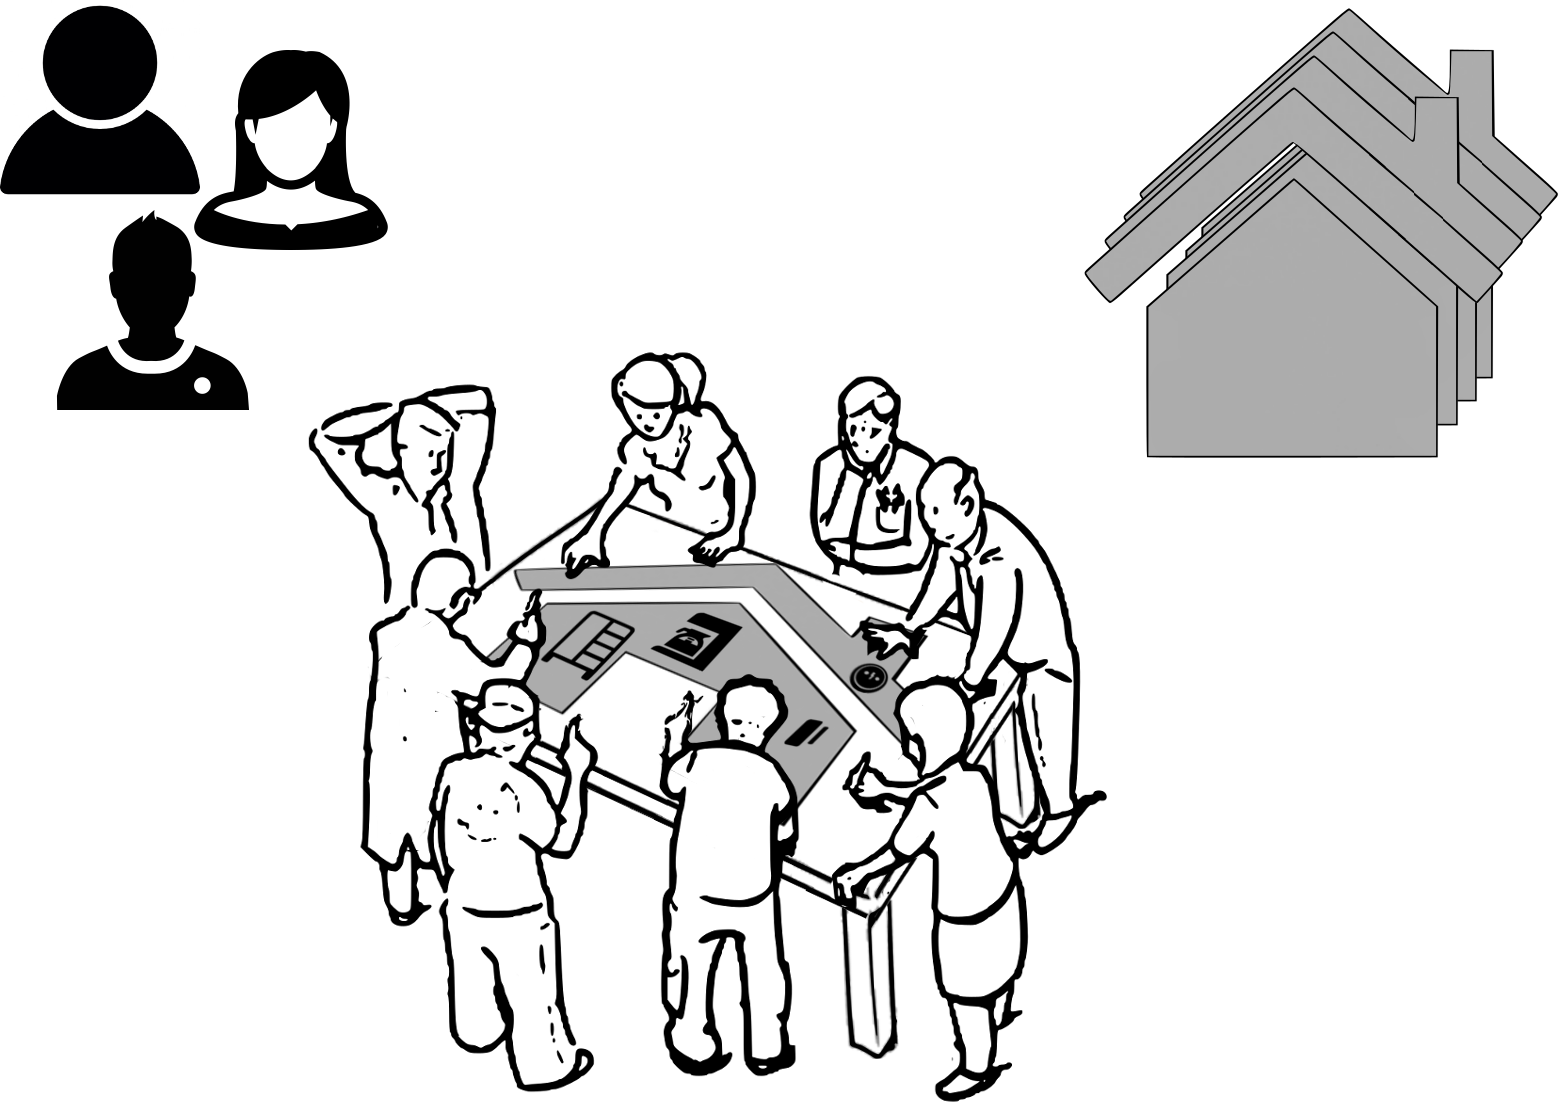
\includegraphics[scale=0.1]{axe_variation_3.png}
\end{minipage}
%\vfill
% \onslide<2->{
%
  \begin{coloredbox}[red]{Problématique}
\centering
   Comment couvrir les besoins des services sensibles au contexte?
  \end{coloredbox}
% }
\end{frame}

% \begin{frame}{Défis de l'autonomie domiciliaire}
% \begin{minipage}{.4\linewidth}
% \onslide<1->{
% \small
%   %\begin{itemize}
% %  \item 
% Fiabilité de la détection du contexte. %liée à l'acceptabilité.
% %  \item 
% \\
% Multiples axes de variation 
% \begin{scriptsize}
% (Utilisateurs, domiciles, intervenants).
% \end{scriptsize}
%   %\item Différents intervenants.% pour définir les services (assistance, maintenance).
%   %\item Différents services.% et objectifs de services (Surveillance de petit-déjeuner, batterie de capteurs, surveillance du réseau).
%   %\item Différentes configurations de domiciles.
%   %\item 

% Dynamicité.
%   %\end{itemize}
% } 
% \end{minipage}
% \hfill
% \begin{minipage}{.5\linewidth}
% \onslide<2->{
%     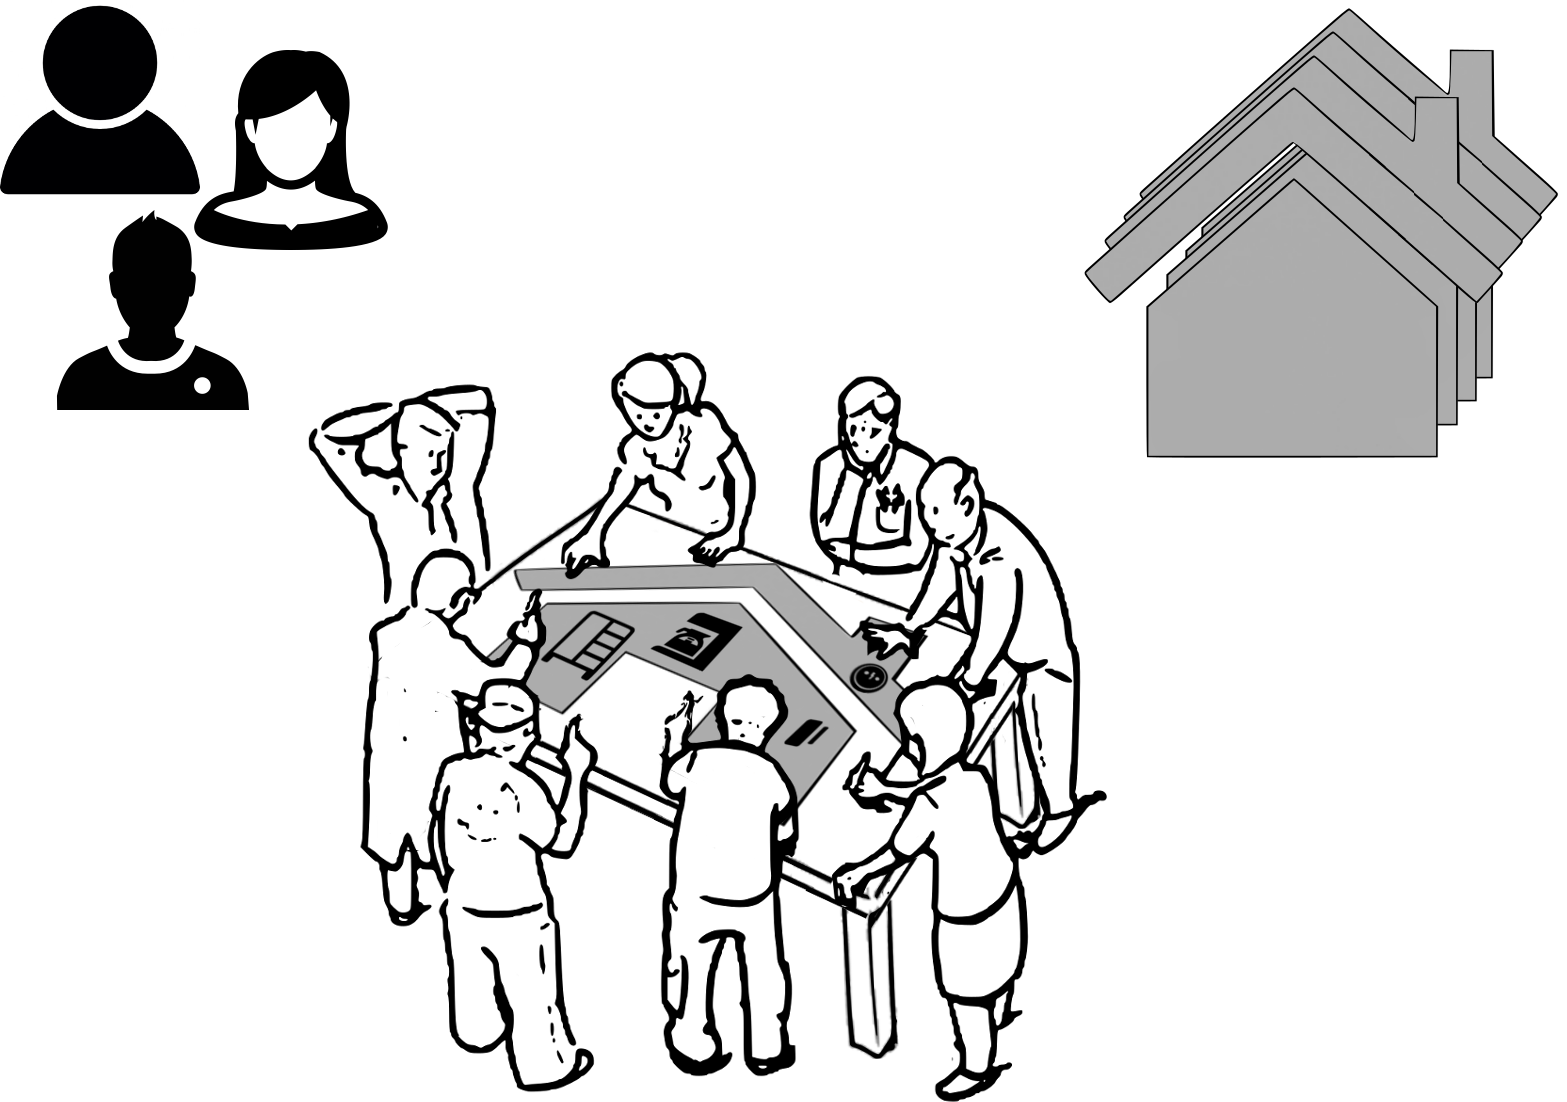
\includegraphics[scale=0.1]{axe_variation0.png}
% }
% \end{minipage}
% \vfill
% \onslide<2->{
%   \begin{coloredbox}[red]{Problématique}
% \centering
%    Comment couvrir les besoins des services sensibles au contexte?
%   \end{coloredbox}
% }
% \end{frame}

% \begin{frame}{Problématique}
%   \begin{coloredbox}[red]{Comment couvrir les besoins de l'autonomie domiciliaire des personnes âgées ?}
%     \begin{itemize}
%     \item Fiabilité de la sensibilité au contexte.
%     \item Différents intervenants.
%     \item Réactivité.
%     \item Passage à l'échelle. %\notespeech{(many homes, many users, many users needs)}.
%     \end{itemize}
%   \end{coloredbox}
% \end{frame}

\begin{frame}{État de l'art}
  Fiabilité de la sensibilité au contexte~:\\
  \begin{itemize}
  \item Simulation de contexte~\cite{bruno2009diasim}.
    \begin{itemize}[label=--,font=\LARGE \color{black}]
    \item Limité aux couches applicatives.
    \end{itemize}
  \item Placement de capteurs~\cite{hong2013toward,murao2013evaluation,beckmann2004some}.
    \begin{itemize}[label=--,font=\LARGE \color{black}]
    \item Intrusifs (caméra, capteurs portés).
    \item Usage en laboratoire (Gants RFID).
    %\item Principes théoriques sans méthodes systématiques.
    \end{itemize}
  \end{itemize}

\end{frame}
\begin{frame}{État de l'art}
  Intervenants~:
  \begin{itemize}
  \item Programmation par les utilisateurs~\cite{resnick2009scratch,coutaz2016first,criel2011deconstructing}.
    \begin{itemize}[label=--,font=\LARGE \color{black}]
    \item Expressivité limitée.
    \item Généralistes.
    \end{itemize}
  \item Services d'assistance domiciliaire~\cite{hoque2015holmes,lee2015sensor,baecker2014technology}.
    \begin{itemize}[label=--,font=\LARGE \color{black}]
    \item Approches en silo.
    \end{itemize}
  \end{itemize}
  %Scaling-up~:\\

  Réactivité~:
  \begin{itemize}
  \item Approches de traitement événementiel~\cite{cugola2012processing}.
    \begin{itemize}[label=--,font=\LARGE \color{black}]
    \item Complexe à mettre en {\oe}uvre.
    \end{itemize}
  \end{itemize}
\end{frame}

\begin{frame}{Thèse~: Unifier l'expression des contextes.}
%\begin{center}
 % \begin{itemize}
    \onslide<1->{
%    \item 
\hspace{50mm}
Modèle d'infrastructure% pour la fiabilité de la sensibilité au contexte.
      \begin{itemize}[label=$\rightarrow$,font=\LARGE \color{red}]
      \item \begin{center}Fiabilité.\end{center}
      \end{itemize}
    }
\vfill
    \onslide<2->{
%    \item 
\hspace{50mm}
Langage dédié.
\hspace{50mm}
      \begin{itemize}[label=$\rightarrow$,font=\LARGE \color{red}]
      %\item Passage à l'échelle.
      \item \begin{center}Axes de variation.\end{center}
      \end{itemize}
    }
\vfill
    \onslide<3->{
%    \item 
\hspace{50mm}
Paradigme événementiel.
\hspace{50mm}
      \begin{itemize}[label=$\rightarrow$,font=\LARGE \color{red}]
      \item \begin{center}Dynamicité.\end{center}
      \end{itemize}
    }

  %\end{itemize}
%\end{center}
\end{frame}

% \begin{frame}{Thèse~: Unifier l'expression des contextes.}
% \begin{minipage}{.4\linewidth}
% \begin{coloredbox}[red]{}
%   \begin{itemize}
%   \item Fiabilité.
%   \item Passage à l'échelle, différents intervenants.
%   \item Temps réel.
%   \end{itemize}
% \end{coloredbox}
% \end{minipage}
% \hfill
% \begin{minipage}{.55\linewidth}
% \begin{coloredbox}[blue]{}
%   \begin{itemize}
%   \item Modèle d'infrastructure pour la fiabilité de la sensibilité au contexte.
%   \item Approche unifiée avec un langage dédié.
%   \item Approche implantée utilisant un paradigme événementiel
%   \end{itemize}
% \end{coloredbox}
% \end{minipage}
% Domicile sensible au contexte fiable\\
% Approche dirigée par les évènements et unifiée\\
% \vfill
% Approche unifiée avec un langage dédié\\
% Approche implantée utilisant un paradigme événementiel\\
% Validation\\
% Modèle d'infrastructure pour la fiabilité de la sensibilité au contexte


% Need of a reliable context-awareness home \\
% to provide an event-driven and unified approach\\
% \vfill
% unified approach with a domain specific language\\
% implemented approach using event-driven paradigm\\
% validation\\
% infrastructure model to ensure context-awareness reliability

%\end{frame}
